\subsection{Experiment Setup}

% \begin{figure*}[t]
%     \centering
%     \begin{subfigure}[t]{0.5\textwidth}
%         \centering
%         \includegraphics[width=0.95\textwidth]{figures/design-processes/high-len-ordered.png}
%         \caption{High leniency}
%     \end{subfigure}%
%     \begin{subfigure}[t]{0.5\textwidth}
%         \centering
%          \includegraphics[width=0.95\textwidth]{figures/design-processes/low-len-ordered.png}
%         \caption{Low leniency}
%     \end{subfigure}
%     \begin{subfigure}[t]{0.5\textwidth}
%         \centering
%         \includegraphics[width=0.95\textwidth]{figures/design-processes/high-lin-ordered.png}
%         \caption{high lin}
%     \end{subfigure}%
%     \begin{subfigure}[t]{0.5\textwidth}
%         \centering
%          \includegraphics[width=0.95\textwidth]{figures/design-processes/high-mesopat-ordered.png}
%         \caption{High meso pat}
%     \end{subfigure}
%     \caption{Rooms used for the experiments}
% \end{figure*}

% Needs to be clear these 3 points: adaptability, stability, benefits from interaction. 


% \begin{table*}[]
% \centering
% \caption{Results from the four metrics in all scenarios across the 21 dimension pairs. Higher scores per column are highlighted in bold. $\star$ marks the lower values. Average and confidence interval per column are shown in the last row.}\smallskip
% \label{tab:resultsTabla}
% \renewcommand\arraystretch{1.2}
% \resizebox{\textwidth}{!}{%
% \begin{tabular}{|l|cccc|cccc|cccc|cccc|}
% \hline
% Dimensions & \multicolumn{4}{c|}{High Leniency Scenario} & \multicolumn{4}{c|}{Low Leniency Scenario} & \multicolumn{4}{c|}{High Linearity Scenario} & \multicolumn{4}{c|}{High Meso-Pattern Scenario} \\ \hline
%  & \multicolumn{1}{c|}{$\Diamond$} & \multicolumn{1}{c|}{$\bigtriangleup$} & \multicolumn{1}{c|}{$\dagger$} & \multicolumn{1}{c|}{$\bigcirc$} &
%  \multicolumn{1}{c|}{$\Diamond$} & \multicolumn{1}{c|}{$\bigtriangleup$} & \multicolumn{1}{c|}{$\dagger$} & \multicolumn{1}{c|}{$\bigcirc$} &
%  \multicolumn{1}{c|}{$\Diamond$} & \multicolumn{1}{c|}{$\bigtriangleup$} & \multicolumn{1}{c|}{$\dagger$} & \multicolumn{1}{c|}{$\bigcirc$} &
%  \multicolumn{1}{c|}{$\Diamond$} & \multicolumn{1}{c|}{$\bigtriangleup$} & \multicolumn{1}{c|}{$\dagger$} & \multicolumn{1}{c|}{$\bigcirc$} \\ \hline

% Len-Lin & 62.5\% & 2.84\% & 35.03\% & 0.892 & 63.6\% & 3.98\% & 34.24\% & 0.911 & 67.1\% & 1.97\% & 31.63\% & 0.869 & {$^{\star}$50.8\%} & 1.66\% & 30.59\% & 0.914 \\ \hline
% Len-Meso & 78.7\% & 3.02\% & \textbf{39.07\%} & 0.907 & 56.6\% & 2.09\% & 21.15\% & 0.91 & 73.8\% & 1.75\% & 22.93\% & 0.874 & 73\% & 2.62\% & 32.21\% & 0.923 \\ \hline
% Len-Spa & 66\% & 1.89\% & 24.70\% & 0.911 & 64.9\% & 1.76\% & {$^{\star}$18.82\%} & 0.898 & 65.5\% & 0.87\% & {$^{\star}$15.36\%} & 0.894 & 70.7\% & 1.36\% & 23.47\% & 0.917 \\ \hline
% Lin-Meso & 77.9\% & 2.73\% & \textbf{45.35\%} & 0.891 & \textbf{78.7\%} & 2.76\% & \textbf{46.56\%} & 0.894 & 67.2\% & 1.98\% & \textbf{42.40\%} & 0.839 & 71.3\% & 1.68\% & \textbf{45.53\%} & 0.919 \\ \hline
% Lin-Spa & {$^{\star}$\textit{54.6\%}} & {$^{\star}$1.08\%} & 31.32\% & 0.882 & {$^{\star}$52.2\%} & 1.81\% & 27.43\% & 0.898 & 56.5\% & 1.06\% & 31.28\% & 0.839 & {$^{\star}$50.3\%} & {$^{\star}$1.21\%} & 28.70\% & 0.895 \\ \hline
% Meso-Spa & \textbf{91.8\%} & 1.35\% & 34.94\% & 0.897 & \textbf{86.1\%} & {$^{\star}$1.28\%} & 32.19\% & 0.886 & \textbf{77\%} & {$^{\star}$0.27\%} & 21.26\% & 0.875 & \textbf{83.6\%} & 1.23\% & 30.55\% & 0.913 \\ \hline
% Sym-Len & 67.1\% & 2.54\% & 23.01\% & \textbf{0.927} & 62\% & 3.19\% & 20.94\% & \textbf{0.929} & 65.5\% & 1.64\% & 19.14\% & \textbf{0.919} & 59.2\% & 1.32\% & 21.47\% & \textbf{0.934} \\ \hline
% Sym-Lin & 71.5\% & 2.04\% & 37.75\% & 0.906 & 64.1\% & 2.55\% & 30.91\% & 0.909 & \textbf{76.1\%} & 1.82\% & \textbf{35.31\%} & 0.868 & 75.3\% & 2.02\% & \textbf{41.77\%} & 0.916 \\ \hline
% Sym-Meso & \textbf{91\%} & 3.09\% & 36.41\% & 0.913 & 65.6\% & 2.83\% & 23.55\% & 0.912 & 73\% & 1.77\% & 22.58\% & 0.888 & \textbf{83.6\%} & 2.06\% & \textbf{40.27\%} & \textbf{0.933} \\ \hline
% Sym-Spa & 77.2\% & {$^{\star}$1.14\%} & 26.87\% & 0.911 & 75.3\% & {$^{\star}$1.02\%} & 24.13\% & 0.905 & \textbf{77.2\%} & {$^{\star}$0.44\%} & 17.74\% & 0.899 & 76.4\% & {$^{\star}$0.79\%} & 25.78\% & 0.917 \\ \hline
% IS-Len & 58.4\% & 3.98\% & {$^{\star}$20.99\%} & 0.917 & 58.2\% & 5\% & {$^{\star}$19.82\%} & \textbf{0.924} & 58.4\% & 2.49\% & {$^{\star}$17.36\%} & 0.907 & 57.9\% & 3.57\% & {$^{\star}$18.06\%} & 0.924 \\ \hline
% IS-Lin & 64.9\% & \textbf{6.04\%} & 28.03\% & 0.9 & 57.6\% & \textbf{11.35\%} & 22.77\% & 0.919 & 62.5\% & 3.72\% & 25.51\% & 0.881 & 67.1\% & 6.58\% & 30.31\% & 0.921 \\ \hline
% IS-Meso & 69.7\% & 5.27\% & 27.36\% & 0.914 & 68\% & 7.58\% & 29.23\% & 0.909 & 72.1\% & \textbf{4.22\%} & 23.92\% & 0.878 & \textbf{90.2\%} & \textbf{6.81\%} & 36.92\% & 0.928 \\ \hline
% IS-Spa & 75.5\% & 4.57\% & 24.88\% & 0.904 & 70.9\% & 7.57\% & 24.78\% & 0.911 & 75\% & 2.91\% & 19.92\% & 0.892 & 75.5\% & 5.98\% & 25.92\% & 0.919 \\ \hline
% Sim-IS & 55.2\% & 4.53\% & {$^{\star}$19.73\%} & \textit{0.894} & {$^{\star}$48.9\%} & 8.86\% & 20.13\% & 0.908 & 57.9\% & 3.85\% & 18.69\% & 0.874 & 54.3\% & 6.5\% & {$^{\star}$20.15\%} & 0.9 \\ \hline
% Sim-Len & 59.3\% &	2.53$\pm$1.95 &	24.86$\pm$3.209 &	0.89$\pm$0.009 & 55.4\% & 3.61\% & 20.87\% & 0.898 & {$^{\star}$53\%} & 2.09\% & 19.58\% & 0.867 & 54.6\% & 1.83\% & 22.40\% & 0.895 \\ \hline
% Sim-Lin & 55.2\% & 2.66\% & 29.12\% & {$^{\star}$0.872} & 52.7\% & 3.51\% & 29.77\% & 0.886 & 56.2\% & 2.28\% & 25.97\% & {$^{\star}$0.834} & 59.8\% & 3.16\% & 34.26\% & 0.875 \\ \hline
% Sim-Meso & 59\% & 3.21\% & 25.65\% & 0.881 & 62.3\% & 3.13\% & 30.27\% & {$^{\star}$0.88} & 68\% & 1.72\% & 26.90\% & {$^{\star}$0.836} & 70.5\% & 3.06\% & 34.08\% & 0.899 \\ \hline
% Sim-Spa & 63.6\% & 1.89\% & 25.17\% & 0.881 & 61.4\% & 2.08\% & 25.13\% & {$^{\star}$0.883} & 66.3\% & 1.04\% & 22.64\% & 0.842 & 64.7\% & 1.99\% & 24.56\% & {$^{\star}$0.885} \\ \hline
% Sym-IS & 72.6\% & \textbf{5.93\%} & 21.64\% & \textbf{0.92} & 64.7\% & \textbf{9.97\%} & 21.11\% & \textbf{0.932} & 75.3\% & \textbf{4.37\%} & 20.02\% & \textbf{0.918} & 73.4\% & \textbf{6.92\%} & 25.01\% & \textbf{0.934} \\ \hline
% Sym-Sim & 60.3\% & 2.48\% & 24.22\% & 0.887 & 56.8\% & 4.77\% & 22.55\% & 0.901 & 67.4\% & 2.18\% & 20.97\% & 0.867 & 64.1\% & 2.45\% & 24.56\% & 0.893 \\ \hline

% Avg. & 67.9$\pm$4.66 & 3.1$\pm$0.61 & 28.8$\pm$2.86 &  0.9$\pm$0.01 & 
% 63.1$\pm$3.79 & 4.3$\pm$1.25 & 26$\pm$2.73 & 0.9$\pm$0.01 &
% 67.2$\pm$3.14 & 2.1$\pm$0.48 & 23.9$\pm$2.76 & 0.87$\pm$0.01 &
% 67.9$\pm$4.66 & 3.1$\pm$0.88 & 29.4$\pm$3.09 & 0.91$\pm$0.01 \\ \hline

% \multicolumn{17}{l}{$\Diamond$ Total explored space\ \
% $\bigtriangleup$ Average growth of explored space per step} \\ 
% \multicolumn{17}{l}{ $\dagger$  Average explored space among all steps \ \
% $\bigcirc$ Average population fitness throughout all generations}
% \end{tabular}%
% }
% \end{table*}



% \begin{table*}
% \begin{subtable}[t]{0.48\textwidth}
% \begin{tabular}[t]{@{} l c *{2}{d{1.7}} @{}}
% \toprule
%  Band &   L & \mc{$\mathcal{O}_{JK}^2$} & \mc{$\mathcal{O}_{EP}^2$} \\
% \midrule
%   1 &   0 &      0.97470(3) &       0.9881(3) \\
% \midrule                                                  
%      &   2 &      0.8290(2)  &       0.882(2)  \\
%      &   3 &      0.96595(4) &       0.979(1)  \\
%   2 &   4 &      0.95328(6) &       0.9736(8) \\
%      &   5 &      0.98727(2) &       0.9950(10)\\
%      &   6 &      0.9168(1)  &       0.950(1)  \\
% \midrule                                                  
%      &   0 &      0.7776(4) &       0.8685(8) \\
%      &   1 &      0.96289(5)&       0.971(2)  \\
%      &   2 &      0.8385(2) &       0.8838(8) \\
%      &   3 &      0.9021(1) &       0.929(1)  \\
%      &   4 &      0.8687(2) &       0.9079(7) \\
%   3 &   5 &      0.9382(1) &       0.946(3)  \\
%      &   6 &      0.9052(2) &       0.9401(4) \\
%      &   7 &      0.9198(2) &       0.9483(5) \\
%      &   8 &      0.9649(5) &       0.9763(4) \\
%      &   9 &      0.9502(1) &       0.971(2)  \\
%      &  10 &      0.9126(3) &       0.941(2)  \\
% \bottomrule
% \end{tabular}
% \caption{\footnotesize (10,15)}
% \label{tab:table1_a}
% \end{subtable}
% \hspace{\fill}
% \begin{subtable}[t]{0.48\textwidth}
% \flushright
% \begin{tabular}[t]{@{} l c *{2}{d{1.7}} @{}}
% \toprule
%  Band &  L & \mc{$\mathcal{O}_{JK}^2$} & \mc{$\mathcal{O}_{EP}^2$} \\ 
% \midrule
%   1 &  0 &      0.997120(3) &      0.9987(2) \\
% \midrule                                                  
%      &  2 &      0.97193(2) &      0.9830(7)  \\
%   2 &  3 &      0.93118(5) &      0.9542(7)  \\
%      &  4 &      0.92257(8) &      0.9486(7)  \\
%      &  5 &      0.98844(1) &      0.9937(6)  \\
% \midrule                                                  
%      &  0 &      0.8450(1) &       0.905(2)   \\
%      &  1 &      0.6931(3) &       0.726(2)   \\
%      &  2 &      0.8618(1) &       0.8945(5)  \\
%      &  3 &      0.90250(9)&       0.9233(9)  \\
%   3 &  4 &      0.8487(1) &       0.8839(6)  \\
%      &  5 &      0.9145(1) &       0.9382(7)  \\
%      &  6 &      0.8884(2) &       0.9174(5)  \\
%      &  7 &      0.9572(1) &       0.978(1)   \\
%      &  8 &      0.97651(6)&       0.977(1)   \\
% \bottomrule
% \end{tabular}
% \caption{\footnotesize (9,16)}
% \label{tab:table1_b}
% \end{subtable}

% \bigskip 

% \begin{subtable}[t]{0.48\textwidth}
% \begin{tabular}[t]{@{} l c *{2}{d{1.7}} @{}}
% \toprule
%  Band &    L & \mc{$\mathcal{O}_{JK}^2$} & \mc{$\mathcal{O}_{EP}^2$} \\
% \midrule                                                    
%   1 &  2.5 &      0.97230(3) &      0.9866(6) \\
% \midrule                                                    
%      &  1.5 &      0.96685(6) &      0.980(3)  \\
%      &  2.5 &      0.92390(9) &      0.956(4)  \\
%      &  3.5 &      0.9075(3)  &      0.9403(5) \\
%   2 &  4.5 &      0.9256(4)  &      0.9541(4) \\
%      &  5.5 &      0.9920(3)  &      0.9957(5) \\
%      &  6.5 &      0.97562(4) &      0.984(1)  \\
%      &  7.5 &      0.9358(1)  &      0.963(2)  \\
% \bottomrule
% \end{tabular}
% \caption{\footnotesize (9,13)}
% \label{tab:table1_c}
% \end{subtable}
% \hspace{\fill}
% \begin{subtable}[t]{0.48\textwidth}
% \flushright
% \begin{tabular}[t]{@{} l c *{2}{d{1.7}} @{}}
% \toprule
%  Band &  L & \mc{$\mathcal{O}_{JK}^2$} & \mc{$\mathcal{O}_{EP}^2$} \\
% \midrule                                                 
%      &  1 &        0.97285(3) &      0.9834(9)  \\
%   1 &  3 &        0.89744(10)&      0.9298(10) \\
%      &  5 &        0.97480(3) &      0.9863(6)  \\
% \midrule                                                  
%      &  1 &      0.8590(3) &      0.915(1)   \\
%      &  2 &      0.8428(4) &      0.8925(8)  \\
%      &  3 &      0.8859(5) &      0.9195(8)  \\
%   2 &  4 &      0.8799(1) &      0.9139(10) \\
%      &  5 &      0.8939(3) &      0.9216(9)  \\
%      &  6 &      0.9587(2) &      0.9752(9)  \\
%      &  7 &      0.9286(1) &      0.9541(8)  \\
%      &  8 &      0.94937(5)&      0.965(2)   \\
% \bottomrule
% \end{tabular}
% \caption{\footnotesize (10,16)}
% \label{tab:table1_d}
% \end{subtable}



% \caption{\footnotesize Main caption describing \subref{tab:table1_a}, \subref{tab:table1_b}, \subref{tab:table1_c} and \subref{tab:table1_d}.}
% \label{tab:table1}
% \end{table*}



% Please add the following required packages to your document preamble:
% \usepackage{graphicx}
% Please add the following required packages to your document preamble:
% \usepackage{graphicx}
\begin{table}[t!]
\centering
\resizebox{0.7\textwidth}{!}              & $^{\star}${19.46$\pm$5.55}     & \textbf{0.96$\pm$0.013}    \\ \hline
Len-Spa    & 71.4\%                          & $^{\star}${19.34$\pm$7.979}    & 0.94$\pm$0.016             \\ \hline
Lin-Meso   & 78.7\%                          & \textbf{43.5$\pm$3.76}         & 0.92$\pm$0.013             \\ \hline
Lin-Spa    & $^{\star}${57.8\%}              & 28.28$\pm$4.109                & 0.92$\pm$0.011             \\ \hline
Meso-Spa   & \textbf{78.9\%}                 & 27.15$\pm$7.315                & 0.93$\pm$0.012             \\ \hline
Sym-Len    & 68.1\%                          & 21.54$\pm$5.88                 & \textbf{0.97$\pm$0.014}    \\ \hline
Sym-Spa    & \textbf{83.4\%}                 & 24.87$\pm$10.334               & 0.95$\pm$0.014             \\ \hline
Sim-Lin    & 58.4\%                          & 30.78$\pm$2.602                & $^{\star}${0.9$\pm$0.012}  \\ \hline
Sim-Meso   & 62.3\%                          & 27.98$\pm$3.385                & $^{\star}${0.9$\pm$0.014}  \\ \hline
Sym-IS     & 70.8\%                          & 21.63$\pm$3.877                & \textbf{0.96$\pm$0.011}    \\ \hline
Average.   & 67.09$\pm$3.35                  & 25.75$\pm$2.48                 & 0.93$\pm$0.01              \\ \hline \hline
Dimensions & \multicolumn{3}{c|}{High Linearity Scenario}                                                  \\ \hline
           & \multicolumn{1}{c|}{$\Diamond$} & \multicolumn{1}{c|}{$\dagger$} & $\bigcirc$                 \\ \hline
Len-Spa    & 72.6\%                          & $^{\star}${16.31$\pm$3.035}    & 0.91$\pm$0.006             \\ \hline
Lin-Meso   & 67.2\%                          & \textbf{40.79$\pm$3.221}       & 0.85$\pm$0.015             \\ \hline
Lin-Spa    & 62.7\%                          & 33.55$\pm$0.963                & $^{\star}${0.84$\pm$0.013} \\ \hline
Sym-Len    & 72.6\%                          & 20.5$\pm$2.646                 & \textbf{0.94$\pm$0.008}    \\ \hline
Sym-Lin    & \textbf{84.3\%}                 & \textbf{37.94$\pm$2.103}       & 0.87$\pm$0.013             \\ \hline
Sym-Spa    & \textbf{85.5\%}                 & 18.94$\pm$4.366                & 0.92$\pm$0.011             \\ \hline
Sim-Len    & $^{\star}${58.7\%}              & 20.93$\pm$2.174                & 0.87$\pm$0.011             \\ \hline
Sim-Lin    & 62.3\%                          & 27.78$\pm$1.424                & $^{\star}${0.84$\pm$0.014} \\ \hline
Sim-Meso   & 68\%                            & 25.6$\pm$1.946                 & $^{\star}${0.84$\pm$0.011} \\ \hline
Sym-IS     & 82.8\%                          & 21.24$\pm$3.005                & \textbf{0.94$\pm$0.011}    \\ \hline
Average.   & 71.8$\pm$3.12                   & 24.52$\pm$2.81                 & 0.89$\pm$0.01              \\ \hline \hline
Dimensions & \multicolumn{3}{c|}{High Meso-Pattern Scenario}                                               \\ \hline
           & \multicolumn{1}{c|}{$\Diamond$} & \multicolumn{1}{c|}{$\dagger$} & $\bigcirc$                 \\ \hline
Len-Lin    & $^{\star}${56.3\%}              & 32.49$\pm$1.536                & 0.92$\pm$0.007             \\ \hline
Lin-Spa    & $^{\star}${55.7\%}              & 30.47$\pm$1.959                & 0.9$\pm$0.007              \\ \hline
Sym-Len    & 65.7\%                          & $^{\star}${22.73$\pm$5.025}    & \textbf{0.96$\pm$0.009}    \\ \hline
Sym-Lin    & 83.4\%                          & \textbf{44.4$\pm$1.019}        & 0.93$\pm$0.007             \\ \hline
Sym-Meso   & 83.6\%                          & 38.45$\pm$5.136                & \textbf{0.96$\pm$0.01}     \\ \hline
IS-Meso    & \textbf{90.2\%}                 & 34.82$\pm$3.749                & 0.95$\pm$0.009             \\ \hline
Sim-IS     & 59.9\%                          & $^{\star}${21.16$\pm$2.237}    & 0.91$\pm$0.009             \\ \hline
Sim-Lin    & 66.3\%                          & 36.29$\pm$1.585                & $^{\star}${0.89$\pm$0.008} \\ \hline
Average.   & 72.34$\pm$4.12                  & 29.88$\pm$2.84                 & 0.93$\pm$0.01              \\ \hline
\end{tabular}%
}
\caption{Results from the three metrics in all scenarios across the relevant dimension pairs. $\Diamond$ relates to coverage, $\dagger$ relates to average coverage per step, and $\bigcirc$ average population fitness throughout all generations. Higher scores per column are highlighted in bold. $\star$ marks the lower values. Confidence intervals are shown for each average value ($\dagger$, and $\bigcirc$), and in the last row we show the average of all the 21 dimensions per metric and scenario.}
\label{tab:resultsTable}
\end{table}

% \begin{table}[]
% \begin{tabular}{|l|ccc}
% \hline
% Dimensions & \multicolumn{3}{c|}{\textit{High Leniency Scenario}}                                                                    \\ \hline
%         & \multicolumn{1}{c|}{$\Diamond$}  & \multicolumn{1}{c|}{$\dagger$} & \multicolumn{1}{c|}{$\bigcirc$}          \\ \hline
% Lin-Meso   & 77.9\%                           & \textbf{43.05$\pm$2.974\textbf{ & 0.9$\pm$0.007                            \\ \hline
% Meso-Spa   & \textbf{84.2\%\} & 30.38$\pm$3.796                           & 0.92$\pm$0.01                            \\ \hline
% Sym-Len    & 74.4\%                           & 24.38$\pm$3.527                           & \textbackslash{}textbf\{0.94$\pm$0.008\} \\ \hline
% Sym-Lin    & 79.2\%                           & \textbackslash{}textbf\{40.14$\pm$2.302\} & 0.91$\pm$0.007                           \\ \hline
% Sym-Meso   & \textbackslash{}textbf\{91\%\}   & 34.37$\pm$3.976                           & 0.93$\pm$0.009                           \\ \hline
% Sym-Spa & \textbackslash{}textbf\{85.5\%\} & 28.47$\pm$5.985                & \textbackslash{}textbf\{0.94$\pm$0.009\} \\ \hline
% Sim-IS     & 60.8\%                           & $^{\star}$\{20.71$\pm$1.687\}             & 0.9$\pm$0.007                            \\ \hline
% Sim-Len    & $^{\star}$\{59.3\%\}             & 24.86$\pm$3.209                           & 0.89$\pm$0.009                           \\ \hline
% Sim-Lin    & 61.1\%                           & 30.8$\pm$1.256                            & $^{\star}$\{0.88$\pm$0.005\}             \\ \hline
% Sim-Meso   & $^{\star}$\{59\%\}               & 24.2$\pm$2.542                            & 0.89$\pm$0.011                           \\ \hline
% Sym-IS     & 78.9\%                           & 22.74$\pm$2.85                            & \textbackslash{}textbf\{0.94$\pm$0.012\} \\ \hline
% Average.   & 72.19$\pm$3.97                   & 29.2$\pm$2.59                             & 0.91$\pm$0.01                           
% \end{tabular}
% \end{table}

% \begin{table*}[t]
% \centering
% \caption{Results from the four metrics in all scenarios across the 21 dimension pairs. Higher scores per column are highlighted in bold. $\star$ marks the lower values. Confidence intervals are shown for each average value ($\bigtriangleup$, $\dagger$, and $\bigcirc$), and in the last row.}\smallskip
% \label{tab:resultsTable}
% \renewcommand\arraystretch{1.2}
% \resizebox{\textwidth}{!}{%
% \begin{tabular}{|l|cccc|cccc|cccc|cccc|}
% \hline
% Dimensions & \multicolumn{4}{c|}{High Leniency Scenario} & \multicolumn{4}{c|}{Low Leniency Scenario} & \multicolumn{4}{c|}{High Linearity Scenario} & \multicolumn{4}{c|}{High Meso-Pattern Scenario} \\ \hline
%  & \multicolumn{1}{c|}{$\Diamond$} & \multicolumn{1}{c|}{$\bigtriangleup$} & \multicolumn{1}{c|}{$\dagger$} & \multicolumn{1}{c|}{$\bigcirc$} &
%  \multicolumn{1}{c|}{$\Diamond$} & \multicolumn{1}{c|}{$\bigtriangleup$} & \multicolumn{1}{c|}{$\dagger$} & \multicolumn{1}{c|}{$\bigcirc$} &
%  \multicolumn{1}{c|}{$\Diamond$} & \multicolumn{1}{c|}{$\bigtriangleup$} & \multicolumn{1}{c|}{$\dagger$} & \multicolumn{1}{c|}{$\bigcirc$} &
%  \multicolumn{1}{c|}{$\Diamond$} & \multicolumn{1}{c|}{$\bigtriangleup$} & \multicolumn{1}{c|}{$\dagger$} & \multicolumn{1}{c|}{$\bigcirc$} \\ \hline

% Len-Lin &
%   69.3\% &
%   2.84$\pm$1.864 &
%   37.25$\pm$2.978 &
%   0.9$\pm$0.01 &
%   70.5\% &
%   3.98$\pm$2.864 &
%   35.4$\pm$2.039 &
%   0.93$\pm$0.011 &
%   74.4\% &
%   1.97$\pm$1.406 &
%   33.96$\pm$1.826 &
%   0.87$\pm$0.013 &
%   $^{\star}${56.3\%} &
%   1.66$\pm$1.559 &
%   32.49$\pm$1.536 &
%   0.92$\pm$0.007 \\ \hline
% Len-Meso &
%   78.7\% &
%   3.02$\pm$2.514 &
%   37.02$\pm$3.686 &
%   0.93$\pm$0.012 &
%   $^{\star}${56.6\%} &
%   2.09$\pm$1.679 &
%   $^{\star}${19.46$\pm$5.55} &
%   \textbf{0.96$\pm$0.013} &
%   73.8\% &
%   1.75$\pm$1.389 &
%   21.84$\pm$3.129 &
%   0.89$\pm$0.013 &
%   73\% &
%   2.62$\pm$1.852 &
%   30.82$\pm$3.728 &
%   0.95$\pm$0.009 \\ \hline
% Len-Spa &
%   73.2\% &
%   1.89$\pm$1.702 &
%   26.13$\pm$4.871 &
%   0.93$\pm$0.01 &
%   71.4\% &
%   1.7$\pm$1.371 &
%   $^{\star}${19.34$\pm$7.979} &
%   0.94$\pm$0.016 &
%   72.6\% &
%   0.87$\pm$0.609 &
%   $^{\star}${16.31$\pm$3.035} &
%   0.91$\pm$0.006 &
%   78.3\% &
%   1.36$\pm$2.041 &
%   24.82$\pm$7.167 &
%   0.95$\pm$0.01 \\ \hline
% Lin-Meso &
%   77.9\% &
%   2.73$\pm$1.928 &
%   \textbf{43.05$\pm$2.974} &
%   0.9$\pm$0.007 &
%   78.7\% &
%   2.76$\pm$2.623 &
%   \textbf{43.5$\pm$3.76} &
%   0.92$\pm$0.013 &
%   67.2\% &
%   1.98$\pm$1.349 &
%   \textbf{40.79$\pm$3.221} &
%   0.85$\pm$0.015 &
%   71.3\% &
%   1.68$\pm$1.252 &
%   43.61$\pm$2.225 &
%   0.93$\pm$0.008 \\ \hline
% Lin-Spa &
%   60.5\% &
%   $^{\star}${1.08$\pm$0.672} &
%   33.26$\pm$1.986 &
%   0.89$\pm$0.007 &
%   $^{\star}${57.8\%} &
%   1.81$\pm$1.776 &
%   28.28$\pm$4.109 &
%   0.92$\pm$0.011 &
%   62.7\% &
%   1.06$\pm$0.677 &
%   33.55$\pm$0.963 &
%   $^{\star}${0.84$\pm$0.013} &
%   $^{\star}${55.7\%} &
%   1.21$\pm$0.71 &
%   30.47$\pm$1.959 &
%   0.9$\pm$0.007 \\ \hline
% Meso-Spa &
%   \textbf{84.2\%} &
%   1.35$\pm$1.177 &
%   30.38$\pm$3.796 &
%   0.92$\pm$0.01 &
%   \textbf{78.9\%} &
%   $^{\star}${1.27$\pm$0.831} &
%   27.15$\pm$7.315 &
%   0.93$\pm$0.012 &
%   70.7\% &
%   $^{\star}${0.27$\pm$0.254} &
%   18.46$\pm$3.768 &
%   0.9$\pm$0.006 &
%   75.2\% &
%   1.24$\pm$1.151 &
%   27.48$\pm$5.656 &
%   0.95$\pm$0.009 \\ \hline
% Sym-Len &
%   74.4\% &
%   2.54$\pm$1.382 &
%   24.38$\pm$3.527 &
%   \textbf{0.94$\pm$0.008} &
%   68.1\% &
%   3.18$\pm$2.733 &
%   21.54$\pm$5.88 &
%   \textbf{0.97$\pm$0.014} &
%   72.6\% &
%   1.64$\pm$0.736 &
%   20.5$\pm$2.646 &
%   \textbf{0.94$\pm$0.008} &
%   65.7\% &
%   1.32$\pm$1.235 &
%   $^{\star}${22.73$\pm$5.025} &
%   \textbf{0.96$\pm$0.009} \\ \hline
% Sym-Lin &
%   79.2\% &
%   2.04$\pm$1.664 &
%   \textbf{40.14$\pm$2.302} &
%   0.91$\pm$0.007 &
%   71.1\% &
%   2.55$\pm$1.684 &
%   31.99$\pm$3.057 &
%   0.93$\pm$0.01 &
%   \textbf{84.3\%} &
%   1.82$\pm$1.703 &
%   \textbf{37.94$\pm$2.103} &
%   0.87$\pm$0.013 &
%   83.4\% &
%   2.02$\pm$1.487 &
%   \textbf{44.4$\pm$1.019} &
%   0.93$\pm$0.007 \\ \hline
% Sym-Meso &
%   \textbf{91\%} &
%   3.09$\pm$2.023 &
%   34.37$\pm$3.976 &
%   0.93$\pm$0.009 &
%   65.6\% &
%   2.83$\pm$1.656 &
%   21.51$\pm$4.894 &
%   0.95$\pm$0.015 &
%   73\% &
%   1.77$\pm$1.326 &
%   21.46$\pm$2.058 &
%   0.9$\pm$0.007 &
%   83.6\% &
%   2.06$\pm$1.899 &
%   38.45$\pm$5.136 &
%   \textbf{0.96$\pm$0.01} \\ \hline
% Sym-Spa &
%   \textbf{85.5\%} &
%   $^{\star}${1.14$\pm$0.979} &
%   28.47$\pm$5.985 &
%   \textbf{0.94$\pm$0.009} &
%   \textbf{83.4\%} &
%   $^{\star}${1.02$\pm$1.214} &
%   24.87$\pm$10.334 &
%   0.95$\pm$0.014 &
%   \textbf{85.5\%} &
%   $^{\star}${0.44$\pm$0.331} &
%   18.94$\pm$4.366 &
%   0.92$\pm$0.011 &
%   84.6\% &
%   $^{\star}${0.79$\pm$0.977} &
%   27.28$\pm$6.95 &
%   0.95$\pm$0.012 \\ \hline
% IS-Len &
%   63.9\% &
%   3.97$\pm$3.0142 &
%   22.06$\pm$2.111 &
%   0.93$\pm$0.011 &
%   62\% &
%   4.81$\pm$4.172 &
%   20.31$\pm$3.445 &
%   0.95$\pm$0.011 &
%   63.9\% &
%   2.48$\pm$1.764 &
%   18.38$\pm$2.458 &
%   0.92$\pm$0.014 &
%   63.9\% &
%   3.6$\pm$3.068 &
%   18.98$\pm$3.073 &
%   0.93$\pm$0.009 \\ \hline
% IS-Lin &
%   71.7\% &
%   \textbf{6.11$\pm$4.379} &
%   29.53$\pm$1.758 &
%   0.91$\pm$0.01 &
%   63.3\% &
%   \textbf{11.42$\pm$14.689} &
%   23.37$\pm$2.573 &
%   0.94$\pm$0.012 &
%   69\% &
%   3.75$\pm$1.936 &
%   27.16$\pm$1.996 &
%   0.89$\pm$0.014 &
%   74.4\% &
%   6.64$\pm$8.471 &
%   32.02$\pm$2.139 &
%   0.93$\pm$0.007 \\ \hline
% IS-Meso &
%   68\% &
%   5.35$\pm$2.838 &
%   25.44$\pm$3.892 &
%   0.93$\pm$0.009 &
%   66.4\% &
%   7.71$\pm$8.917 &
%   26.74$\pm$3.154 &
%   0.93$\pm$0.012 &
%   72.1\% &
%   \textbf{4.37$\pm$2.464} &
%   22.45$\pm$3.026 &
%   0.9$\pm$0.014 &
%   \textbf{90.2\%} &
%   \textbf{7.04$\pm$7.66} &
%   34.82$\pm$3.749 &
%   0.95$\pm$0.009 \\ \hline
% IS-Spa &
%   82.2\% &
%   4.53$\pm$2.762 &
%   26.17$\pm$3.235 &
%   0.92$\pm$0.01 &
%   78\% &
%   7.58$\pm$10.187 &
%   25.46$\pm$5.17 &
%   0.93$\pm$0.012 &
%   82.5\% &
%   2.92$\pm$1.932 &
%   21.14$\pm$2.654 &
%   0.91$\pm$0.012 &
%   83.1\% &
%   6.01$\pm$6.755 &
%   27.3$\pm$3.288 &
%   0.94$\pm$0.009 \\ \hline
% Sim-IS &
%   60.8\% &
%   4.57$\pm$2.033 &
%   $^{\star}${20.71$\pm$1.687} &
%   0.9$\pm$0.007 &
%   53.9\% &
%   8.97$\pm$11.514 &
%   20.63$\pm$2.849 &
%   0.93$\pm$0.013 &
%   63.9\% &
%   3.89$\pm$1.934 &
%   19.82$\pm$2.225 &
%   0.88$\pm$0.014 &
%   59.9\% &
%   6.59$\pm$7.01 &
%   $^{\star}${21.16$\pm$2.237} &
%   0.91$\pm$0.009 \\ \hline
% Sim-Len &
%   $^{\star}${59.3\%} &
%   2.53$\pm$1.95 &
%   24.86$\pm$3.209 &
%   0.89$\pm$0.009 &
%   60.8\% &
%   3.55$\pm$3.249 &
%   21.56$\pm$3.774 &
%   0.92$\pm$0.013 &
%   $^{\star}${58.7\%} &
%   2.09$\pm$1.054 &
%   20.93$\pm$2.174 &
%   0.87$\pm$0.011 &
%   60.5\% &
%   1.83$\pm$2.135 &
%   23.71$\pm$4.175 &
%   0.91$\pm$0.011 \\ \hline
% Sim-Lin &
%   61.1\% &
%   2.66$\pm$2.046 &
%   30.8$\pm$1.256 &
%   $^{\star}${0.88$\pm$0.005} &
%   58.4\% &
%   3.51$\pm$4.411 &
%   30.78$\pm$2.602 &
%   $^{\star}${0.9$\pm$0.012} &
%   62.3\% &
%   2.28$\pm$1.971 &
%   27.78$\pm$1.424 &
%   $^{\star}${0.84$\pm$0.014} &
%   66.3\% &
%   3.16$\pm$3.281 &
%   36.29$\pm$1.585 &
%   $^{\star}${0.89$\pm$0.008} \\ \hline
% Sim-Meso &
%   $^{\star}${59\%} &
%   3.21$\pm$2.345 &
%   24.2$\pm$2.542 &
%   0.89$\pm$0.011 &
%   62.3\% &
%   3.13$\pm$3.072 &
%   27.98$\pm$3.385 &
%   $^{\star}${0.9$\pm$0.014} &
%   68\% &
%   1.72$\pm$1.03 &
%   25.6$\pm$1.946 &
%   $^{\star}${0.84$\pm$0.011} &
%   70.5\% &
%   3.06$\pm$2.157 &
%   32.32$\pm$2.134 &
%   0.92$\pm$0.014 \\ \hline
% Sim-Spa &
%   70.5\% &
%   1.89$\pm$1.597 &
%   26.66$\pm$3.252 &
%   0.89$\pm$0.01 &
%   68.1\% &
%   2.08$\pm$2.648 &
%   25.99$\pm$5.582 &
%   0.91$\pm$0.014 &
%   73.5\% &
%   1.04$\pm$0.541 &
%   24.21$\pm$2.569 &
%   0.85$\pm$0.011 &
%   71.4\% &
%   1.97$\pm$2.189 &
%   25.99$\pm$4.479 &
%   0.91$\pm$0.013 \\ \hline
% Sym-IS &
%   78.9\% &
%   \textbf{5.91$\pm$3.455} &
%   22.74$\pm$2.85 &
%   \textbf{0.94$\pm$0.012} &
%   70.8\% &
%   \textbf{9.98$\pm$10.962} &
%   21.63$\pm$3.877 &
%   \textbf{0.96$\pm$0.011} &
%   82.8\% &
%   \textbf{4.39$\pm$2.644} &
%   21.24$\pm$3.005 &
%   \textbf{0.94$\pm$0.011} &
%   81\% &
%   \textbf{6.96$\pm$7.55} &
%   26.36$\pm$3.488 &
%   0.95$\pm$0.008 \\ \hline
% Sym-Sim &
%   66.6\% &
%   2.5$\pm$1.813 &
%   25.64$\pm$3.739 &
%   0.9$\pm$0.008 &
%   62.7\% &
%   4.81$\pm$6.691 &
%   23.26$\pm$4.408 &
%   0.93$\pm$0.015 &
%   74.4\% &
%   2.2$\pm$1.271 &
%   22.45$\pm$2.078 &
%   0.88$\pm$0.013 &
%   70.8\% &
%   2.47$\pm$2.459 &
%   25.98$\pm$4.003 &
%   0.91$\pm$0.012 \\ \hline
% Average. &
%   72.19$\pm$3.97 &
%   3.09$\pm$0.62 &
%   29.2$\pm$2.59 &
%   0.91$\pm$0.01 &
%   67.09$\pm$3.35 &
%   4.32$\pm$1.26 &
%   25.75$\pm$2.48 &
%   0.93$\pm$0.01 &
%   71.8$\pm$3.12 &
%   2.13$\pm$0.49 &
%   24.52$\pm$2.81 &
%   0.89$\pm$0.01 &
%   72.34$\pm$4.12 &
%   3.11$\pm$0.9 &
%   29.88$\pm$2.84 &
%   0.93$\pm$0.01 \\ \hline

% \multicolumn{17}{l}{$\Diamond$ Total explored space\ \
% $\bigtriangleup$ Average growth of explored space per step} \\ 
% \multicolumn{17}{l}{ $\dagger$  Average explored space among all steps \ \
% $\bigcirc$ Average population fitness throughout all generations}
% \end{tabular}%
% }
% \end{table*}

% \begin{table}[h!]
% \centering
% % \renewcommand\arraystretch{1.2}
% \resizebox{0.48\textwidth}{!}{%
% \begin{tabular}{l|llll}
% \multicolumn{1}{|l|}{Dimension} & \multicolumn{1}{c|}{$\Diamond$} & \multicolumn{1}{c|}{$\bigtriangleup$} & \multicolumn{1}{c|}{$\dagger$} & \multicolumn{1}{c|}{$\bigcirc$}  \\ \hline

% Len  & 67.58±2.68 & 2.47±0.39 & 24.78±2.45 & 0.93±0.01 \\
% Lin  & 68.62±3.3  & 3.03±0.89 & 34.49±2.28 & 0.9±0.01  \\
% Meso & 73.16±3.43 & 2.84±0.69 & 29.95±3.1  & 0.92±0.01 \\
% Spa  & 74.56±3.49 & 1.94±0.68 & 25.75±1.71 & 0.92±0.01 \\
% Sym  & 76.63±3.1  & 2.89±0.85 & 27.01±2.77 & 0.93±0.01 \\
% Sim  & 64.32±2.16 & 3.15±0.67 & 25.39±1.61 & 0.89±0.01 \\
% IS   & 71.11±3.68 & 5.81±0.87 & 23.98±1.64 & 0.93±0.01 \\ \hline

% \multicolumn{5}{l}{$\Diamond$ Total explored space} \\ 
% \multicolumn{5}{l}{
% $\bigtriangleup$ Average growth of explored space per step} \\ 
% \multicolumn{5}{l}{ $\dagger$  Average explored space among all steps} \\
% \multicolumn{5}{l}{$\bigcirc$ Average population fitness throughout all generations}

% \end{tabular}%
% }%
% \caption{Summary and average per dimension used in table~\ref{tab:resultsTable}. Confidence intervals are shown per value.}%
% \label{tab:perDimension}
% \end{table}

%In our experiments, we discuss and analyze two desirable features in QD-algorithms, \textit{stability} and \textit{adaptability}. %, and fertility~\citepninth{p9Ashlock2018-fertility}, 
%as two features to be analyzed. 

\begin{figure*}[t!]
\centerline{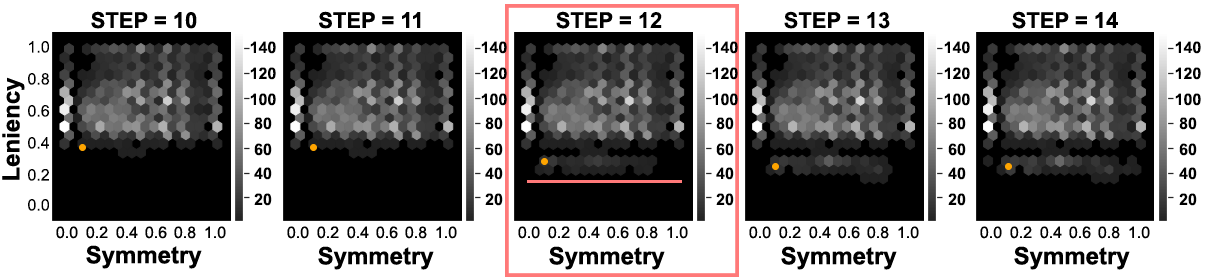
\includegraphics[width=\textwidth]{figures/exp1-lowlen-exploring_new_area/accumulative__X-sym-Y-len-simplified-2.png}}
%\centerline{\includegraphics[width=0.55\textwidth]{figures/low-len/accu__X-sym-Y-len.png}}
\caption{Aggregated TERA using Sym and Len following the low leniency scenario (fig.~\ref{figs:roomsexperiments}.a). Highlights how the design introduces new generative region to the algorithm. In red (step 12) it is highlighted when the design enters a new region of the space and MAP-Elites is then able to generate individuals in that region, explained in detail in Case 1.}
\label{figs:exp1}
\end{figure*}

We have conducted a series of experiments on EDD to analyze the \emph{adaptability} and \emph{stability} of IC MAP-Elites, as well as the effects of the interaction for MAP-Elites and the user. \emph{Stability} relates to the steady generation of high-performing individuals, while gradually growing the search and stably covering the generative space at each edit step. \emph{Adaptability} relates to the ability of the search to adapt to changing conditions, adjusting the search to the new goals, while still generating high-performing individuals. Both features, relate to the notions of evolvability~\citepninth{p9doncieux2020-noveltyEvolvability}, the ability of the search to generate creative individuals in problems with changing conditions.

% as how the search process benefits from the continuous mixed-initiative approach. 

We recorded three different design sessions, called scenarios, where we manually designed, step by step, dungeon rooms with specific target design goals. They are shown in Figure~\ref{figs:roomsexperiments}: a) a boss room - identified as a \textbf{low leniency} design goal; b) a linear room with specific paths and targets - identified as a \textbf{high linearity} design goal, and finally, c) a room where each chamber within is usable - identified as a \textbf{high meso-pattern} design goal. We chose these design goals as they represent key metrics with clear distinct representative goals and design styles that one might create in a dungeon.

% (Figure~\ref{figs:roomsexperiments}): a) low leniency, b) high linearity, and c) high meso-pattern level. 

% , e.g., (a) a final boss room, (b) a linear room with specific paths and targets, and (c) a room where each chamber within is usable; all 3 named in relation to their “associated” dimension. The goals relate to the dimensions because dimensions are orthogonal to some extent to the fitness function in MAP-Elites, which in the case of the dimensions in EDD, make them closer to properties you would aim for when creating levels .e.g., leniency or linearity. Each edition is included as-is in the population and used as a target in the fitness function by IC MAP-Elites, updating corridor, chamber, and inventorial ratios affecting the quality of micro and meso patterns. 

%  Each scenario was run under every combination of EDD's feature-dimensions in pairs ($21$), where the dimensions are
The experiments consist on running these pre-recorded scenarios separately on EDD, step by step with a lapse of $100$ evolutionary generations between steps. Each scenario implies 21 evolutionary runs, one per each pair of feature-dimension, where the dimensions are (table~\ref{tab:dimensions}): leniency (len), linearity (lin), spatial patterns (spa), meso-patterns (meso), symmetry (sym), similarity (sim), and inner similarity (IS). Each edition (i.e., design step) is included as-is in the population and used as a target in the fitness function by IC MAP-Elites, updating corridor, chamber, and inventorial ratios affecting the quality of micro and meso patterns. Every $100$ generations we collect the novel generated individuals to later analyze how the search and the fitness landscape vary after each design step. Step after step, we measure how the explored generative space grows, as well as how distribution and concentration of elites together with the manually edited room traverse the generative space.%, while keeping track of all individuals' fitness scores. 

% (i.e., if the algorithm generates an individual previously generated, we do not 


In all the experiments, the initial population was set to $1000$ mutated individuals. All cells were set to a maximum capacity of $25$ individuals each. In every generation, we selected $5$ cells random, and $5$ parents per cell through tournament selection. The random selection followed a uniform distribution. Offspring were produced through a two-point crossover and a $30$\% mutation chance. Using this setup, between $150$ to $2001$ individuals were produced every $100$ generations, with an average of $373$ unique individuals generated every $100$ generations throughout all runs.

\subsubsection{Metrics}

All our experiments are evaluated and analyzed following the same procedure and metrics, focusing in the novel generated individuals. In particular, we calculated the \textit{coverage} ($\Diamond$), the \textit{average coverage per step} ($\dagger$), and \textit{average fitness} ($\bigcirc$). \textit{Coverage} relates to the percentage of space covered by the search in total and is calculated as the cumulative amount of covered hexagons at the final step divided by the maximum amount in our experiments. \textit{Average coverage} relates to the average coverage per step, i.e., how much of the space is covered at each design step in average, calculated as the cumulative coverage per step divided by the amount of design editions. Finally, \textit{average fitness} calculates the average individual fitness in the search throughout all generations.



% the \textit{cumulative coverage average among all design steps} .

\begin{figure*}[t!]
\centerline{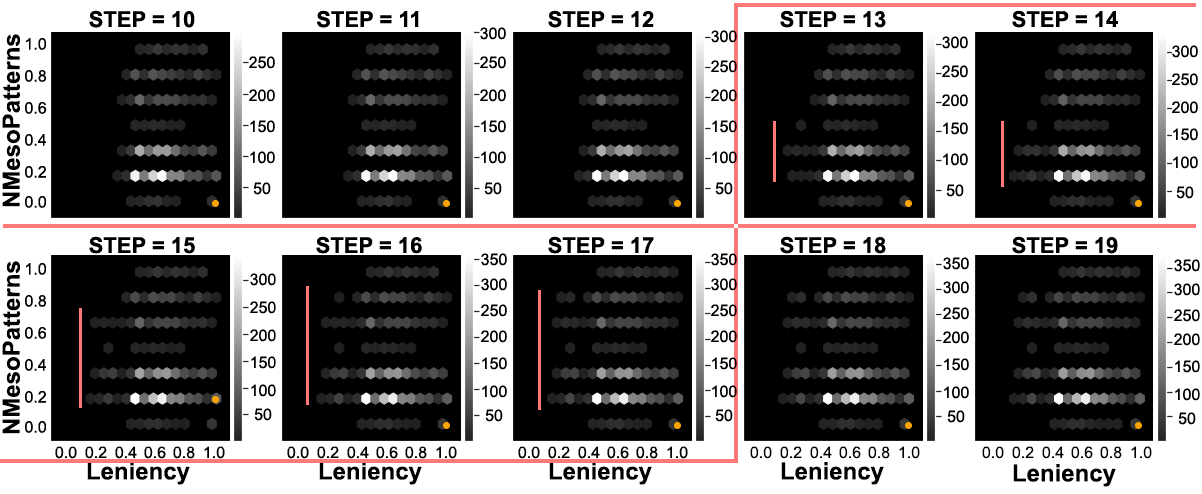
\includegraphics[width=\textwidth]{figures/exp2-highlin-exploringchamber/accumulative__X-len-Y-mesoPat-simplify-2.png}}
%\centerline{\includegraphics[width=0.55\textwidth]{figures/low-len/accu__X-sym-Y-len.png}}
\caption{Aggregated TERA using Len and Meso following the high linearity scenario (fig.~\ref{figs:roomsexperiments}.b). Highlights subtle discovery of new generative regions.  In red (step 12), this subtle discovery is highlighted, explained in detail in Case 2.}
\label{figs:exp2}
\end{figure*}

\subsection{Results and Analysis}

% - Table 2 is included to both serve as a guide for the reader to assess the multiple evaluations done per scenario, and to show the algorithms stability to cover the space while encountering high-performing individuals (QD-properties); thus, the algorithm adapts to the new editions which change the fitness landscape. The first column shows the algorithm’s coverage supported by the second column, which shows that in average MAP-Elites keep exploring and generating novel levels and is not just sporadically generating novel levels. The last column presents the average final fitness by summing the novel levels’ fitnesses after every step (100 generations). Short confidence intervals show that the average numbers do not rely on outliers and that the averages show stable behaviors. Further, table 2 shows an extract of all the pair of dimensions, focusing on the ones that showed the lowest or highest values, which is why all the 21 pair of dimensions are not shown. In retrospect, we can see that the information about the table and why is needed should be extended in the paper, which we will extend with a more precise argumentation for its need in the camera-ready version.

Table \ref{tab:resultsTable} shows an extract of all test results. The results were filtered to only show the pair of dimensions with the lowest or highest values in different metrics. This means that some pair of dimensions are not shown since all their metric values were in between lower and higher scores. Each subtable represents one of the three design scenarios, each of them displaying the metrics described above. The higher and lower scores per column are highlighted in bold and with $\star$, respectively. Confidence intervals are shown per value when using averages. In general, table~\ref{tab:resultsTable} shows IC MAP-Elites' stability to cover the space while encountering high-performing individuals; thus, it is able to adapt to the new editios which change the fitness landscape. Coverage ($\Diamond$), supported by average coverage per step ($\dagger$) and average fitness ($\bigcirc$), shows that in average the algorithm keeps exploring and generating novel and high-performing individuals rather than sporadically generating them.

% Total space coverage ($\Diamond$) is calculated as the cumulative amount of covered hexagons at the final step divided by the maximum amount in our experiments. Average of explored space among all design steps ($\dagger$) is the cumulative amount of covered hexagons divided by the amount of design editions. 

% Table \ref{tab:resultsTable} shows a compilation of all test results. The wider columns represent one of the three design scenarios, each of them displaying the following metrics: $\Diamond$, total space coverage ($\%$); $\dagger$, average $\%$ of explored space among all design steps; $\bigcirc$, average fitness throughout all generations. The higher and lower scores per column are highlighted in bold and with $\star$, respectively. Confidence intervals are shown per value when using averages. Total space coverage ($\Diamond$) is calculated as the cumulative amount of covered hexagons at the final step divided by the maximum amount in our experiments. Average of explored space among all design steps ($\dagger$) is the cumulative amount of covered hexagons divided by the amount of design editions. 


The symmetry and spatial pattern (Sym-Spa) dimension pair explore and cover on average more of the space across all scenarios than others ($\Diamond$). In general, when using either \textit{sym} or \textit{spa}, MAP-Elites is pressured to generate content that maximizes the utility of walls since both use walls as a core building block. Similarly, \textit{Meso} and \textit{IS} are two other dimensions that perform well with others, especially~\textit{Meso}. However,~\textit{Meso} requires combination of shapes with walls and correct placement of tiles; thus, in principle involving more complex operations to achieve high dimensional values. % On the other hand, linearity and spatial pattern (Lin-Spa) explores the least. Linearity does not achieve great results in space exploration, except when linearity is the target design goal (case three) or combined with some other more explorative dimension.

 
% The meso- and spatial pattern (Meso-Spa) dimension pair scores the largest explored space ($\Diamond$) in all scenarios, whereas linearity and spatial pattern (Lin-Spa) explores the least in 3 out of 4. Large explored spaces signify that the good synergy between both dimensions enables the underlying evolutionary algorithm to explore most of it. Meso- and spatial pattern align well with each other, since proper placement of spatial patterns is often favorable to the arrangement of meso-patterns. Linearity does not generally (all dimension pairs including Lin) achieve great results in space exploration, except for the third scenario, where linearity is the target design goal. Combinations involving similarity (Sim) explore less the generative space, but this feature implies searching for individuals that are different-yet-close to the manually edited room, therefore the evolutionary process focuses in areas of the generative space around it.

Overall the average population fitness ($\bigcirc$) is very high with 0.915 in average (of a maximum 1.0) with a narrow confidence interval $\pm$0.01. Symmetry and leniency (Sym-Len) scored the highest in all scenarios while Similarity and Linearity (Sim-Lin) scored the lowest. This shows a stable behavior in the IC MAP-Elites as that the average quality of individuals is high even when large portions of the generative space are explored (high diversity), and regardless of the dimension pair chosen. 

% Notice that the average population fitness ($\bigcirc$) is overall very high, with symmetry and leniency (Sym-Len) scoring the highest in all scenarios. This is very relevant, since it shows a stable behaviour in the IC MAP-Elites as that the average quality of individuals is high even when large portions of the generative space are explored (high diversity), and regardless of the dimension pair chosen. 

IC MAP-Elites works in constant interaction with the edited design. Each step reshapes the fitness landscape to a certain extent, which could hinder the evolutionary process. However, per step, an avg. of 27.34\% of the space is covered by generating novel individuals (i.e., not encountered previously in the population). This, coupled with the relatively narrow confidence intervals, means that the search is constantly exploring the space, diversifying and encountering new spaces. However, as it will be exemplified through the cases, the implicit explorative and exploitative mechanisms of MAP-Elites might not be enough to explore new regions, which can be introduced interactively to MAP-Elites.

%Furthermore, the searched space continuously grows after every step ($\bigtriangleup$). The wider confidence interval is due to the big steps performed at earlier generations, which is expected to some extent by MAP-Elites as there is high-pressure to fill the bins with elites. As more elites are encountered, the lesser bins will remain empty; thus, the search will cover similar spaces, which is what can be observed in most of our experiments. Fontaine et al.~\citepninth{p9Fontaine2019-hearhstoneDecks} explored and evaluated a similar scenario with good results using MAP-Elites with Sliding Boundaries. In our experiments, When using \textit{Inner Similarity (IS)}, the search grew the most on average regardless of the second dimension, as well as with \textit{Similarity (Sim)}. \textit{Sim} focuses on aesthetical similarity and \textit{IS} internal similarity regarding sparsity and density of tiles. Thus, this could be due to the dimensions pressuring the search to generate different-yet-close individuals to the target room.

% As more elites are encountered, the lesser bins remain empty 

% IC MAP-Elites works in constant interaction with the human designer. Each step reshapes the fitness landscape to a certain extent, which could hinder the evolutionary process. Nevertheless, the searched space continuously grows after every step ($\bigtriangleup$), showing high levels of adaptability to the designer's choices. The linearity and meso-pattern (Lin-Meso) combination shows the higher average explored space per step ($\dagger$) scores in all scenarios. Despite not covering the vastest spaces, individuals are widespread up to almost half the entire space at every step.

%  The dimensions in the ERAs are the same as the IC MAP-Elites, which means that the ERA is effectively the expressivity of the MAP-Elites grid.
The following cases examine TERAs following the different scenarios presented in figure~\ref{figs:roomsexperiments}. Different cases will use either an aggregated TERA step by step or a non-aggregated version showing each step's specific scores in the evaluated dimensions. Each figure's caption and respective case will indicate what type of TERA is used. Non-Aggregated TERAs show the delta maps in the search, meaning where the search has focused and the space covered for a specific step. On the other hand, aggregated TERAs show the density of generated individuals over all steps and the coverage up to the specific step. In each TERA, we also show as an orange dot where the current design is in relation to the used and tested dimensions. Case 1 and 2 examine aggregated TERAs, while case 3 examines non-agreggated TERAs.

% The following cases examine TERAs following the different scenarios presented in figure~\ref{figs:roomsexperiments}. Different cases will use either an aggregated TERA step by step or a non-aggregated version showing each step's specific scores in the evaluated dimensions. Each figure's caption and respective case will indicate what type of TERA is used. Non-Aggregated TERAs show the delta maps in the search, meaning where the search has focused and the space covered for a specific step. On the other hand, aggregated TERAs show the density over all steps of the generated individuals and the covered space up to the specific step. In each TERA, we also show as an orange dot where the current design is in relation to the used and tested dimensions. Case 1 and 2 examine aggregated TERAs, while case 3 examines non-agreggated TERAs.

%The following cases examine ERAs following the different scenarios presented in figure~\ref{figs:roomsexperiments}. Case 1 and 2, examine ERAs where each step is subsequently aggregated, while case 3 and 4, examine ERAs where each step are the unique individuals generated at each step. 

%non-aggregated ERAs are indeed delta maps showing differences. Specifically, they show where the search has focus and the covered space on the current step. On the other hand, aggregated ERAs show more general information of the expressive range, such as the whole generated space and the density of the generated levels.

% \begin{figure*}[t!]
%     \centering
%     \subfloat[Aggregated TERA using Sym and Len following the low leniency scenario (fig.~\ref{figs:roomsexperiments}.a). Highlights how the design introduces new generative area to the algorithm. In red (step 12) it is highlighted when the design enters a new area of the space and MAP-Elites is then able to generate individuals in that area, explained in detail in Case 1.\label{fig:go}]{%
%       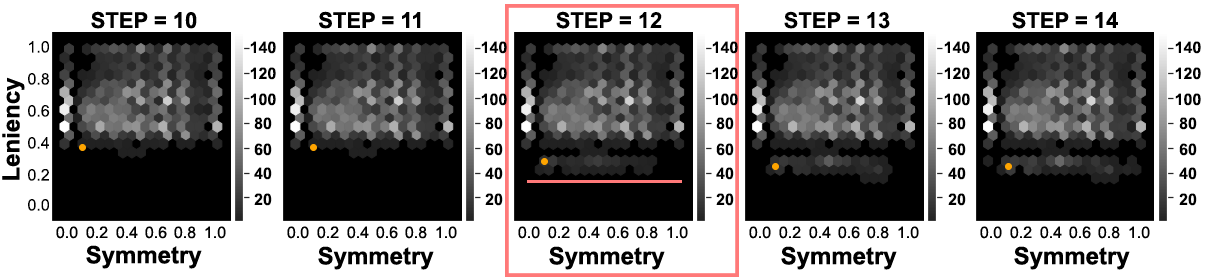
\includegraphics[width=0.8\textwidth]{figures/exp1-lowlen-exploring_new_area/accumulative__X-sym-Y-len-simplified-2.png}
%      }\hfill
%      \subfloat[Aggregated TERA using Len and Meso following the high linearity scenario (fig.~\ref{figs:roomsexperiments}.b). Highlights subtle discovery of new generative areas.  In red (step 12), this subtle discovery is highlighted, explained in detail in Case 2.\label{fig:go}]{%
%       \includegraphics[width=0.8\textwidth]{figures/exp2-highlin-exploringchamber/accumulative__X-len-Y-mesoPat-simplify.png}
%      }\hfill
%     %  \medskip
%      \subfloat[Non-aggregated TERA using Sym and Meso following the high meso-pattern level scenario (fig.~\ref{figs:roomsexperiments}.c). Highlights overall properties of interacting with MAP-Elites. Lighter areas identified with a, b, c, and d, represent the main areas of focus explained in detail in Case 3.\label{fig:scf}]{%
%       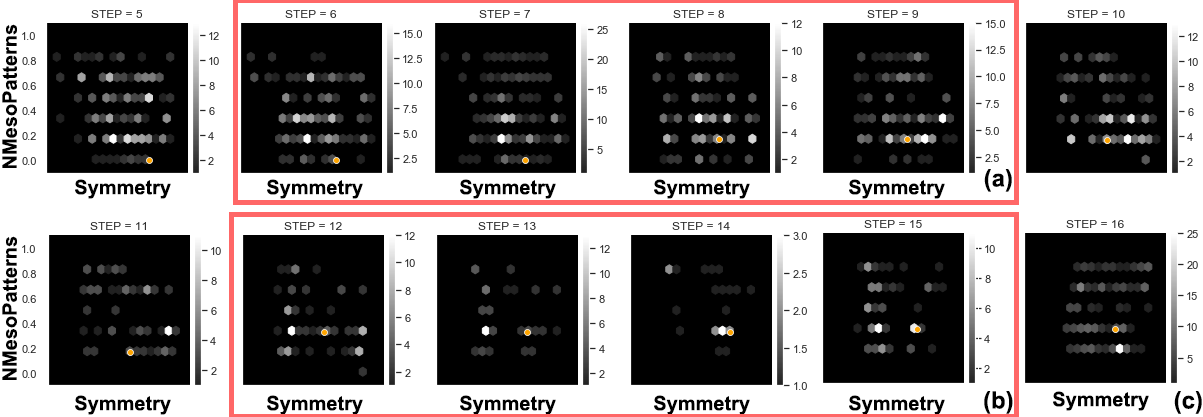
\includegraphics[width=0.8\textwidth]{figures/exp4-mesopat-explorDeadend_leavesearch/simple__X-sym-Y-mesoPat-simplify-combo.png}
%      }
    
%     \caption{Example archetypical paths from different frequent sequences.}
%     \label{fig:archetypical-examples}
% \end{figure*}







\begin{figure*}[ht]
\centerline{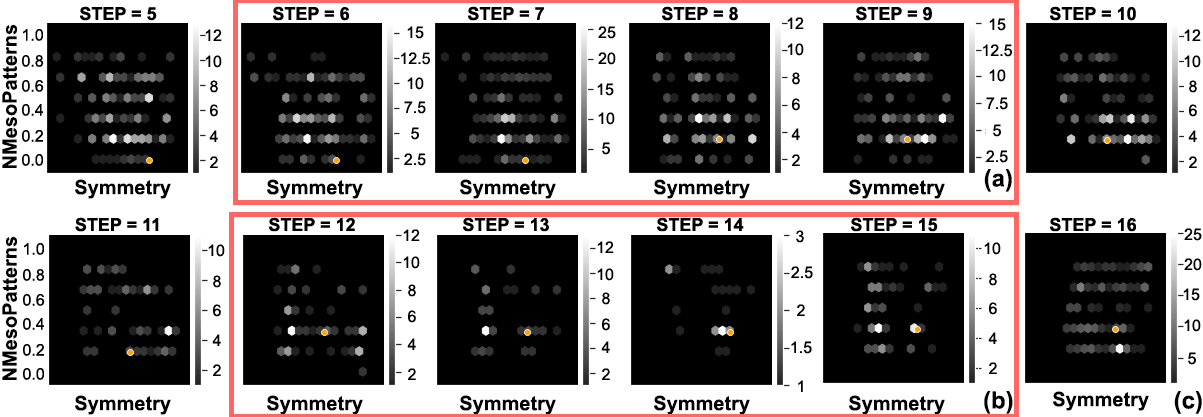
\includegraphics[width=\textwidth]{figures/exp4-mesopat-explorDeadend_leavesearch/simple__X-sym-Y-mesoPat-simplify-combo-2.png}}
%\centerline{\includegraphics[width=0.55\textwidth]{figures/low-len/accu__X-sym-Y-len.png}}
\caption{Non-aggregated TERA using Sym and Meso following the high meso-pattern level scenario (fig.~\ref{figs:roomsexperiments}.c). Highlights overall properties of interacting with MAP-Elites.a, b, and c, represent the main areas of focus explained in detail in Case 3.}
\label{figs:exp3}
\end{figure*}





% \begin{figure*}[t]
% \centerline{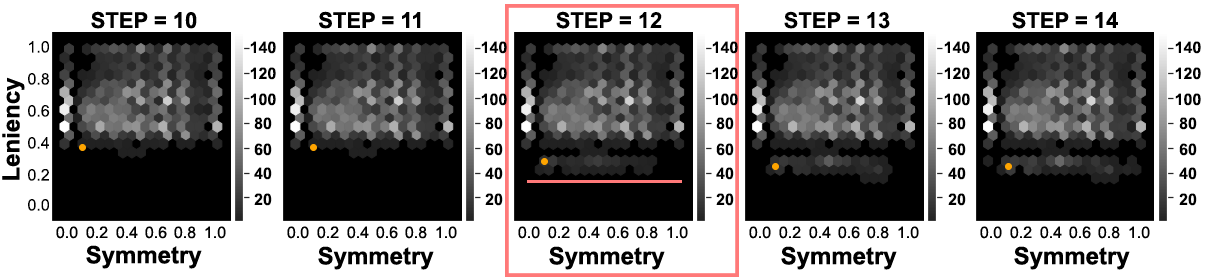
\includegraphics[width=0.8\textwidth]{figures/exp1-lowlen-exploring_new_area/accumulative__X-sym-Y-len-simplified-2.png}}
% %\centerline{\includegraphics[width=0.55\textwidth]{figures/low-len/accu__X-sym-Y-len.png}}
% \caption{Aggregated TERA using Sym and Len following the low leniency scenario (fig.~\ref{figs:roomsexperiments}.a). Highlights how the design introduces new generative area to the algorithm. In red (step 12) it is highlighted when the design enters a new area of the space and MAP-Elites is then able to generate individuals in that area, explained in detail in Case 1.}
% \label{figs:exp1}
% \end{figure*}

% \begin{figure}[h]
% \centerline{\includegraphics[width=0.47\textwidth]{figures/exp2-highlin-exploringchamber/accumulative__X-len-Y-mesoPat-simplify.png}}
% %\centerline{\includegraphics[width=0.55\textwidth]{figures/low-len/accu__X-sym-Y-len.png}}
% \caption{Aggregated TERA using Len and Meso following the high linearity scenario (fig.~\ref{figs:roomsexperiments}.b). Highlights subtle discovery of new generative areas.  In red (step 12), this subtle discovery is highlighted, explained in detail in Case 2.}
% \label{figs:exp2}
% \end{figure}


% \begin{figure}[ht]
% \centerline{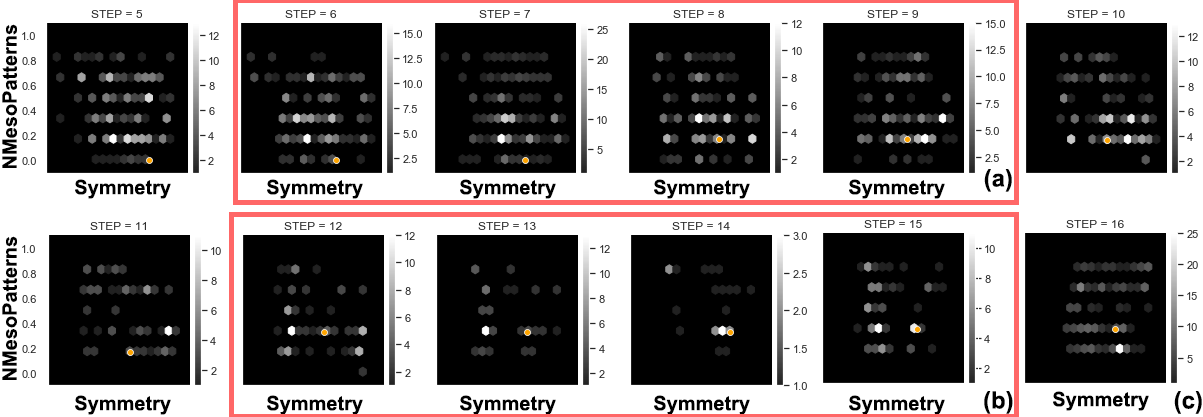
\includegraphics[width=0.47\textwidth]{figures/exp4-mesopat-explorDeadend_leavesearch/simple__X-sym-Y-mesoPat-simplify-combo.png}}
% %\centerline{\includegraphics[width=0.55\textwidth]{figures/low-len/accu__X-sym-Y-len.png}}
% \caption{Non-aggregated TERA using Sym and Meso following the high meso-pattern level scenario (fig.~\ref{figs:roomsexperiments}.c). Highlights overall properties of interacting with MAP-Elites. Lighter areas identified with a, b, c, and d, represent the main areas of focus explained in detail in Case 3.}
% \label{figs:exp3}
% \end{figure}

% \begin{figure*}[t]
%     \centering
%     \begin{subfigure}[t]{0.33\textwidth}
%         \centering
%         \includegraphics[width=0.95\textwidth]{figures/exp5-linearity-Highlen/__X-lin-Y-mesoPat.png}
%         \caption{Linearity-\#MesoPatterns}
%     \end{subfigure}%
%     \begin{subfigure}[t]{0.33\textwidth}
%         \centering
%          \includegraphics[width=0.95\textwidth]{figures/exp5-linearity-Highlen/__X-lin-Y-spaPat.png}
%         \caption{Linearity-\#SpatialPatterns}
%     \end{subfigure}
%     \begin{subfigure}[t]{0.33\textwidth}
%         \centering
%         \includegraphics[width=0.95\textwidth]{figures/exp5-linearity-Highlen/__X-lin-Y-sym.png}
%         \caption{Linearity-Symmetry}
%     \end{subfigure}%
%     \caption{Selected non-Aggregated ERAs using Linearity and following the high leniency scenario (fig.~\ref{figs:roomsexperiments}.a.). The ERAs present pair of dimensions, reusing linearity, where the design remains still for most of the steps in the generative space yet MAP-Elites stably generates novel individuals in a substantial area. Explained in detail in~\ref{sec:case4}.}
%     \label{figs:exp4}
% \end{figure*}

%\subsubsection{Case 1 - Design introducing a new area of the generative space}
\subsubsection{Case 1 - Design Opens New Regions of the Generative Space} \label{sec:case1}

In this case, we analyze the interaction with IC MAP-Elites through examining the generative space when using Sym and Len as dimensions (figure~\ref{figs:exp1}) following the low leniency scenario depicted in figure~\ref{figs:roomsexperiments}.a. The scenario aimed to gradually increase the room's challenge while dividing it into two clear and connected areas.

Table~\ref{tab:resultsTable} shows that this pair of dimensions do not have the best scores except for the $\overline{fitness}$ ($\bigcirc$). This indicates that these dimensions are able to stably find high-performing individuals (above the avg.) while adapting to the new designs exploring an average of 21.54 and a total of 68.1\%. Moreover, in fig~\ref{figs:exp1}, for several steps, half of the generative space is completely unexplored, which could indicate that in those regions, dimensions would be mutually exclusive. 

However, at step 12 (highlighted in red in fig~\ref{figs:exp1}), when reaching a low leniency score, the design enters an unexplored region of the generative space, which subsequently enables IC MAP-Elites to search and generate high-performing individuals in the new region. Furthermore, there is a significant rise in the number of unique individuals generated with a high concentration on the new region, spreading over the already explored space.

\subsubsection{Case 2 - Subtle Changes in the Design Reflected in the Generation of MAP-Elites} \label{sec:case2}

Case 1 showed that by entering an unexplored region of the generative space, the designer could show possibilities for the algorithm and influence the search, yet more subtle guidance is possible. Figure~\ref{figs:exp2} presents such a case. We focus on the high linearity scenario (fig.~\ref{figs:roomsexperiments}.b), where the goal was to create a single narrow corridor between the top and left door and add some objective at the bottom entrance. Through this, we not only aimed at high linearity but also tried to promote other main characteristics such as the open chamber/corridor balance, or the combination of meso-patterns.

Similar to the previous case, in figure~\ref{figs:exp2}, it is shown that for many steps, the search does not explore a big part of the generative space. In this case, the room does not move either in the generative space as the changes are not affecting the dimensions. However, between steps 13 to 17, a new region of the generative space is filled (highlighted in red in fig~\ref{figs:exp2}), which indicates that even if changes in the room do not have a direct influence by moving in the generative space, they still can foster exploration in new regions. These main steps are visible in fig.~\ref{figs:roomsexperiments}.b, subfigure 5, and 6 from the left. Specifically, lower leniency regions are generated once the room is divided into a representative corridor and a big open area with a treasure meso-pattern. These stepping-stones gave the needed “building blocks” to MAP-Elites to cross and mutate until the new generative space was explored. Moreover, similarly to the previous case, the algorithms generates significantly more novel individuals during this time  (around 531 novel individuals), and the search covers 20\% of the space, exploiting the new region, akin to Novelty search behavior~\citepninth{p9liapis2015-ConstrainedNoveltySearch}.

% (the number of novel individuals there is a significant rise in the number of individuals (\~{}531 novel individuals) and a \~{20}\% search grow, concentrating in the new area, akin novelty search's behavior.

%, which is more possible as atleast one of the dimensions matches the design goal of the room. However when

\subsubsection{Case 3 – Exploring Multiple Properties}
\label{sec:case3}

%In case 3, we focus in the high meso-pattern concentration scenario (fig.~\ref{figs:roomsexperiments}.d), where we subdivided the room into small open chambers with clear objectives in them. Furthermore, in this case we analyze the unique individuals generated step by step rather than in an aggregated fashion using Symmetry and \#MesoPatterns as pair of dimensions. 

In this case, we analyze the TERA of unique individuals generated each step using Sym and Meso as dimension pairs (fig.~\ref{figs:exp3}). We heed to the high meso-pattern level scenario (fig.~\ref{figs:roomsexperiments}.c), where we subdivided the room into small open chambers with clear objectives. Overall, in fig.~\ref{figs:exp3} two aspects stand out; firstly, the generative space is explored more at the early steps, as there are fewer constraints from the edited design. Secondly, the generated individuals seem to follow the path taken by the design in the generative space. Supported by the other cases, this indicates that the design can filter the search and point regions of interest for the IC MAP-Elites. %Furthermore,  this pair of dimensions in the specific scenario, have very high scores analyzing the data in table~\ref{tab:resultsTable} for this pair of dimensions in the specific scenario, 

Moreover, opposite to case 1 and as a consequence of filtering the generative space, when the design leaves low scoring regions, the algorithm rapidly disregards creating individuals in those spaces. For instance, the bottom region after step 7 (fig.~\ref{figs:exp3}.a). Further, as the room is changing but without any type of influence in the searched dimensions e.g., steps 12 to 15 (fig.~\ref{figs:exp3}.b), MAP-Elites has difficulties exploring the space. A similar challenge was discussed by Alvarez et al.~\citepninth{p9Alvarez2020-ICMAPE}, where their experiments showed that the search got to a plateau after 1000 generations due to the MAP-Elites lacking the incentive to explore. Even if their experiments focused on static environments, this case gives further evidence that minimal changes to the design and lack of influence in the generative space, conditions the exploration of space and the generation of novel individuals. 

Lastly, at step 16 (fig.~\ref{figs:exp3}.c), we encounter a similar situation as with fig.~\ref{figs:exp2};  where a design edition enables the needed “building blocks” for MAP-Elites. In this case, it was triggered by the forming of a dead-end chamber pattern, which enables even more meso-patterns to be used and discovered. Rather than finding a new region of the generative space, this time, the search gets rebooted, and therefore, explores all regions generating novel individuals.
% Lastly, in the last step of the scenario i.e., step 24 (fig.~\ref{figs:exp3}.d), the design enters the highest score in the meso dimension. Thus, helping MAP-Elites to find individuals in a previously unexplored area akin to fig.~\ref{figs:exp1}.

%\subsubsection{Case 4 - Linearity as a stable dimension}
%\label{sec:case4}

%When Linearity is paired with any other dimension, it seems to constantly explore and generate novel individuals. However, compared to other dimensions, Linearity also reveals more difficulty in adapting and producing higher-quality individuals. 

%It can be observed in table~\ref{tab:resultsTable} that the avg. explored space among all steps ($\dagger$) is generally higher than the rest of the combinations and to the average in most of the scenarios. This indicates that when using Linearity, MAP-Elites steadily generates more unique individuals per step, regardless of the second dimension or the design goal, yielding a robust dimension with a stable search. Although, there are second dimensions, which create a better synergy such as meso. However, a good result in ($\dagger$) does not guarantee a vast exploration of the space nor higher quality individuals, if compared with the rest, as noted in table~\ref{tab:resultsTable} ($\Diamond$) and ($\bigcirc$), respectively. 

%In figure~\ref{figs:exp4}, we present three ERAs where Linearity is paired with other dimensions, in order to highlight its overall influence in the solution space coverage. We focus on the high leniency scenario (fig.~\ref{figs:roomsexperiments}.a), where the aim was to create an initial room with a central challenge, and a side path to avoid such a challenge and collecting treasures in the way. However, when using linearity, the ERAs look akin, which is also reflected in the values of table~\ref{tab:resultsTable}.

%Moreover, this case shows the extensive and stable generation that occurs when using linearity, and even if in most cases, the exploitation is focused on the area of the design, it seems to be detrimental for the algorithm. Simply observing the ERAs, this seems to be caused by the design not moving within the generative space. However, this is recurrent when using linearity regardless of the scenario, which suggests that linearity is a more independent dimension. Therefore, linearity, while making the search more robust and stable, generates less-quality individuals and adapts less to the edited design.

%\subsubsection{Case 4 - Linearity as a stable dimension}
%\label{sec:case4}

%In this case, we are interested in presenting another phenomena and a dimension that while constantly exploring and generating novel individuals, does not adapt nor produce as higher quality as other dimensions. Linearity as a dimension, it

%When Linearity is paired with any other dimension, it seems to constantly explore and generate novel individuals. However, compared to other dimensions, Linearity also reveals more difficulty in adapting and producing higher-quality individuals. 
%but with difficulties in adapting and producing higher-quality individuals than other dimensions.
%Linearity is a dimension that, when used together with any other dimension, seems to constantly explore and generate novel individuals but with difficulties in adapting and producing higher-quality individuals as other dimensions. 
%It can be observed in table~\ref{tab:resultsTable} that the avg. explored space among all steps ($\dagger$) is generally higher than the rest of the combinations and to the average in most of the scenarios. This indicates that when using Linearity, MAP-Elites steadily generates more unique individuals per step, regardless of the second dimension or the design goal, yielding a robust dimension with a stable search. Although, there are second dimensions, which create a better synergy such as meso. However, a good result in ($\dagger$) does not guarantee a vast exploration of the space nor higher quality individuals, if compared with the rest, as noted in table~\ref{tab:resultsTable} ($\Diamond$) and ($\bigcirc$), respectively. 

%Unlike the other cases, in figure~\ref{figs:exp4} we present three ERAs where Linearity is represented with other dimensions to highlight a phenomenon when using linearity. We focus on the high leniency scenario (fig.~\ref{figs:roomsexperiments}.a), where the aim was to create a more introductory room with a central challenge, and a side path to avoid such a challenge and collecting treasures in the way. However, when using linearity, the ERAs look very similar, which is also reflected in the values of table~\ref{tab:resultsTable}. 

%In figure~\ref{figs:exp4}, we present three ERAs where Linearity is paired with other dimensions, in order to highlight its overall influence in the solution space coverage. 
%Unlike the other cases, in figure~\ref{figs:exp4} we present three ERAs where Linearity is represented with other dimensions to highlight a phenomenon when using linearity. 
%We focus on the high leniency scenario (fig.~\ref{figs:roomsexperiments}.a), where the aim was to create an initial room with a central challenge, and a side path to avoid such a challenge and collecting treasures in the way. However, when using linearity, the ERAs look akin%very similar
%, which is also reflected in the values of table~\ref{tab:resultsTable}.

%Moreover, this case shows the extensive and stable generation that occurs when using linearity, and even if in most cases, the exploitation is focused on the area of the design, it seems to be detrimental for the algorithm. Simply observing the ERAs, this seems to be caused by the design not moving within the generative space. However, this is recurrent when using linearity regardless of the scenario, which suggests that linearity is a more independent dimension. Therefore, linearity, while making the search more robust and stable, generates less-quality individuals and adapts less to the edited design.

% \begin{table*}[t]
% \centering
% \caption{I am thinking on having a table were we have all the dimensions and show some percentages on how they "do" in all the different scenarios. For instance, show the percentage of filled space (how much the pair odf dimensions cover the generative space). Another could be to have the average of covered space in all steps }\smallskip
% \begin{tabular}{lcccccccccccccccc}
% Dimensions & a & a & a & a & a & a & a & a & a & a & a & a & a & a & a & a\\ \hline
% a & a & a & a & a & a & a & a & a & a & a & a & a & a & a & a & a\\ \hline
% \end{tabular}
% %}
% \label{table1}
% \end{table*}

% \begin{table*}[t]
% \centering
% \caption{I am thinking on having a table were we have all the dimensions and show some percentages on how they "do" in all the different scenarios. For instance, show the percentage of filled space (how much the pair odf dimensions cover the generative space). Another could be to have the average of covered space in all steps }\smallskip
% \label{tab:resultsTable}
% \renewcommand\arraystretch{1.2}
% \resizebox{\textwidth}{!}{%
% \begin{tabular}{lcccccccccccccccc}
% \hline
% \multicolumn{1}{|l|}{Dimensions} & \multicolumn{4}{c|}{high len} & \multicolumn{4}{c|}{low len} & \multicolumn{4}{c|}{high lin} & \multicolumn{4}{c|}{meso pat} & \multicolumn{4}{c|}{low lin} & \multicolumn{4}{c|}{spat pat} & \multicolumn{4}{c|}{high sym} & \multicolumn{4}{c|}{nylow len} \\ \hline

% \multicolumn{1}{l|}{} & \multicolumn{1}{c|}{$\Diamond$} & \multicolumn{1}{c|}{$\bigtriangleup$} & \multicolumn{1}{c|}{$\box$} & \multicolumn{1}{c|}{$\bigcirc$} & \multicolumn{1}{c|}{$\Diamond$} & \multicolumn{1}{c|}{$\bigtriangleup$} & \multicolumn{1}{c|}{$\box$} & \multicolumn{1}{c|}{$\bigcirc$} & \multicolumn{1}{c|}{$\Diamond$} & \multicolumn{1}{c|}{$\bigtriangleup$} & \multicolumn{1}{c|}{$\box$} & \multicolumn{1}{c|}{$\bigcirc$} & \multicolumn{1}{c|}{$\Diamond$} & \multicolumn{1}{c|}{$\bigtriangleup$} & \multicolumn{1}{c|}{$\box$} & \multicolumn{1}{c|}{$\bigcirc$} & \multicolumn{1}{c|}{$\Diamond$} & \multicolumn{1}{c|}{$\bigtriangleup$} & \multicolumn{1}{c|}{$\box$} & \multicolumn{1}{c|}{$\bigcirc$} & \multicolumn{1}{c|}{$\Diamond$} & \multicolumn{1}{c|}{$\bigtriangleup$} & \multicolumn{1}{c|}{$\box$} & \multicolumn{1}{c|}{$\bigcirc$} & \multicolumn{1}{c|}{$\Diamond$} & \multicolumn{1}{c|}{$\bigtriangleup$} & \multicolumn{1}{c|}{$\box$} & \multicolumn{1}{c|}{$\bigcirc$} & \multicolumn{1}{c|}{$\Diamond$} & \multicolumn{1}{c|}{$\bigtriangleup$} & \multicolumn{1}{c|}{$\box$} & \multicolumn{1}{c|}{$\bigcirc$} \\ \hline


% % & \multicolumn{1}{c|}{b} & \multicolumn{1}{c|}{b} & \multicolumn{1}{c|}{b} & \multicolumn{1}{c|}{b} & \multicolumn{1}{c|}{b} & \multicolumn{1}{c|}{b} & \multicolumn{1}{c|}{b} & \multicolumn{1}{c|}{b} & \multicolumn{1}{c|}{b} & \multicolumn{1}{c|}{b} & \multicolumn{1}{c|}{b} & \multicolumn{1}{c|}{b} & \multicolumn{1}{c|}{b} & \multicolumn{1}{c|}{b} \\ \hline

% \multicolumn{1}{|c|}{Len-Lin} & 62.5\% & 62.5\% & 62.5\% & \multicolumn{1}{c|}{50\%} & 62.5\% & 62.5\% & 62.5\% & \multicolumn{1}{c|}{50\%} & 62.5\% & 62.5\% & 62.5\% & \multicolumn{1}{c|}{50\%} & 62.5\% & 62.5\% & 62.5\% & \multicolumn{1}{c|}{50\%} & 62.5\% & 62.5\% & 62.5\% & \multicolumn{1}{c|}{50\%} & 62.5\% & 62.5\% & 62.5\% & \multicolumn{1}{c|}{50\%} & 62.5\% & 62.5\% & 62.5\% & \multicolumn{1}{c|}{50\%} & 62.5\% & 62.5\% & 62.5\% & \multicolumn{1}{c|}{50\%} \\ \hline

% \multicolumn{17}{l}{$\Diamond$ Total space searched till last design step\ \
% $\bigtriangleup$ Average space searched among all the design steps}
% \end{tabular}%
% }
% \end{table*}